%!TEX program = xelatex
\documentclass[11pt]{beamer}

\usepackage{amsfonts}
\usepackage{amsmath}
\usepackage{blindtext}
\usepackage{enumitem}
\usepackage{hyperref}
\usepackage{colortbl}

\hypersetup{pdfborder = {0 0 0}}

\usetheme{SaoPaulo}

\title{Python Basics!}
\subtitle{dictionaries, mutable arguments}
\author{CS101 Lecture \#11}
\date{2016-09-28}

\setcounter{showSlideNumbers}{1}

\begin{document}
  \setcounter{showProgressBar}{0}
  \setcounter{showSlideNumbers}{0}

%%%%%%%%%%%%%%%%%%%%%%%%%%%%%%%%%%%%%%%%%%%%%%%%%%%%%%%%%%%%%%%%%%%%%%%%%%%%%%%%
\frame{\titlepage}

%%%%%%%%%%%%%%%%%%%%%%%%%%%%%%%%%%%%%%%%%%%%%%%%%%%%%%%%%%%%%%%%%%%%%%%%%%%%%%%%
\setcounter{framenumber}{0}
\setcounter{showProgressBar}{1}
\setcounter{showSlideNumbers}{1}

%%%%%%%%%%%%%%%%%%%%%%%%%%%%%%%%%%%%%%%%%%%%%%%%%%%%%%%%%%%%%%%%%%%%%%%%%%%%%%%%
\section{Administrivia}

%%%%%%%%%%%%%%%%%%%%%%%%%%%%%%%%%%%%%%%%%%%%%%%%%%%%%%%%%%%%%%%%%%%%%%%%%%%%%%%%
\begin{frame}
  \frametitle{Administrivia}
  \Enlarge

  \begin{itemize}
  \myitem  Homework \#5 is due Friday Sep.\ 30.
  \myitem  Midterm \#1 will be Monday Oct.\ 3.  (7 p.m.) \\ \textcolor{CS101GradBot}{No class on Monday, \\ Labs WILL be held all week. \\ Contact \texttt{cs101admin@cs.illinois.edu} for conflict exam.}
  \end{itemize}
\end{frame}

%%%%%%%%%%%%%%%%%%%%%%%%%%%%%%%%%%%%%%%%%%%%%%%%%%%%%%%%%%%%%%%%%%%%%%%%%%%%%%%%
\begin{frame}
  \frametitle{Administrivia}
  \Enlarge

  \begin{tabular}{ll}
  \rowcolor{CS101Alt}
  AYA AYB AYC AYD AYE & \href{http://ada.fs.illinois.edu/0043.html}{Gregory Hall 112} \\ % 369
  \rowcolor{CS101White}
  AYF AYG AYH AYI     & \href{http://ada.fs.illinois.edu/0159.html}{Wohlers Hall 141} \\ % 327
  \rowcolor{CS101Alt}
  AYJ AYK AYL         & \href{http://ada.fs.illinois.edu/0041.html}{Main Library 66} \\ % 216
  \rowcolor{CS101White}
  AYM AYN AYO         & \href{http://ada.fs.illinois.edu/0563.html}{Siebel Center 1404} \\ % 200
  \rowcolor{CS101Alt}
  AYP AYQ AYR         & \href{http://ada.fs.illinois.edu/0054.html}{David Kinley Hall 114} \\ % 280
  \end{tabular}
\end{frame}

%%%%%%%%%%%%%%%%%%%%%%%%%%%%%%%%%%%%%%%%%%%%%%%%%%%%%%%%%%%%%%%%%%%%%%%%%%%%%%%%
\begin{frame}
  \frametitle{Midterm Instructions}
  \Enlarge

  \begin{itemize}
  \myitem  30 multiple-choice questions
  \myitem  60 minutes
  \myitem  Requires NetID and University I-Card.
  \mysubitem  Exams are unique—omitting the exam code will dock one letter grade (10\%).
  \end{itemize}
\end{frame}

%%%%%%%%%%%%%%%%%%%%%%%%%%%%%%%%%%%%%%%%%%%%%%%%%%%%%%%%%%%%%%%%%%%%%%%%%%%%%%%%
\section{Warmup Quiz}

%%%%%%%%%%%%%%%%%%%%%%%%%%%%%%%%%%%%%%%%%%%%%%%%%%%%%%%%%%%%%%%%%%%%%%%%%%%%%%%%
\begin{frame}[fragile]
  \frametitle{Question \#1}
  \Enlarge

  \begin{semiverbatim}
a = [ [1,2,3], [4,5,6], [7,8,9] ]
  \end{semiverbatim}
  How would you refer to the value 8?
  \begin{enumerate}[label=\Alph*]
  \item  \texttt{a[2][3]}
  \item  \texttt{a[1][2]}
  \item  \texttt{a[2,3]}
  \item  \texttt{a[2][1]}
  \end{enumerate}
\end{frame}

%%%%%%%%%%%%%%%%%%%%%%%%%%%%%%%%%%%%%%%%%%%%%%%%%%%%%%%%%%%%%%%%%%%%%%%%%%%%%%%%
\begin{frame}[fragile]
  \frametitle{Question \#2}
  \Enlarge

  \begin{semiverbatim}
x = [ 'a', 'b' ]
y = [ 'c', 'd' ]
def add_it( x,y ):
    y.append( x )
add_it( y,x )
  \end{semiverbatim}
  What is the final value of \texttt{x}?
  \begin{enumerate}[label=\Alph*]
  \item  \texttt{[ 'a', 'b', 'c', 'd' ]}
  \item  \texttt{[ 'a', 'b' ]}
  \item  \texttt{[ 'a', 'b', [ 'c', 'd' ] ]}
  \item  \texttt{None}
  \end{enumerate}
\end{frame}

%%%%%%%%%%%%%%%%%%%%%%%%%%%%%%%%%%%%%%%%%%%%%%%%%%%%%%%%%%%%%%%%%%%%%%%%%%%%%%%%
\begin{frame}[fragile]
  \frametitle{Question \#3}  %TODO:make file i/o question
  \Enlarge

  \begin{semiverbatim}
x = [ 'a', 'b' ]
y = [ 'c', 'd' ]
def add_it( x,y ):
    y.append( x )
add_it( y,x )
  \end{semiverbatim}
  What is the final value of \texttt{x}?
  \begin{enumerate}[label=\Alph*]
  \item  \texttt{[ 'a', 'b', 'c', 'd' ]}
  \item  \texttt{[ 'a', 'b' ]}
  \item  \texttt{[ 'a', 'b', [ 'c', 'd' ] ]}
  \item  \texttt{None}
  \end{enumerate}
\end{frame}

%%%%%%%%%%%%%%%%%%%%%%%%%%%%%%%%%%%%%%%%%%%%%%%%%%%%%%%%%%%%%%%%%%%%%%%%%%%%%%%%
\begin{frame}[fragile]
  \frametitle{Question \#1 (Worked)}
  \Enlarge

  \begin{semiverbatim}
a = 1
def fun(c,b):
    return c + b
a = fun( a,a ) + a
  \end{semiverbatim}
\end{frame}

%%%%%%%%%%%%%%%%%%%%%%%%%%%%%%%%%%%%%%%%%%%%%%%%%%%%%%%%%%%%%%%%%%%%%%%%%%%%%%%%
\section{Dictionaries}

%%%%%%%%%%%%%%%%%%%%%%%%%%%%%%%%%%%%%%%%%%%%%%%%%%%%%%%%%%%%%%%%%%%%%%%%%%%%%%%%
\begin{frame}[fragile]
  \frametitle{\texttt{dict} data type}
  \Enlarge

  \begin{itemize}
  \myitem  How do we index a \texttt{list}?
  \myitem  \texttt{list}s and \texttt{tuple}s are \emph{ordered}.
  \myitem  What else may make sense---how else could you organize data?
  \end{itemize}
\end{frame}

%%%%%%%%%%%%%%%%%%%%%%%%%%%%%%%%%%%%%%%%%%%%%%%%%%%%%%%%%%%%%%%%%%%%%%%%%%%%%%%%
\begin{frame}[fragile]
  \frametitle{Example}
  \Enlarge

  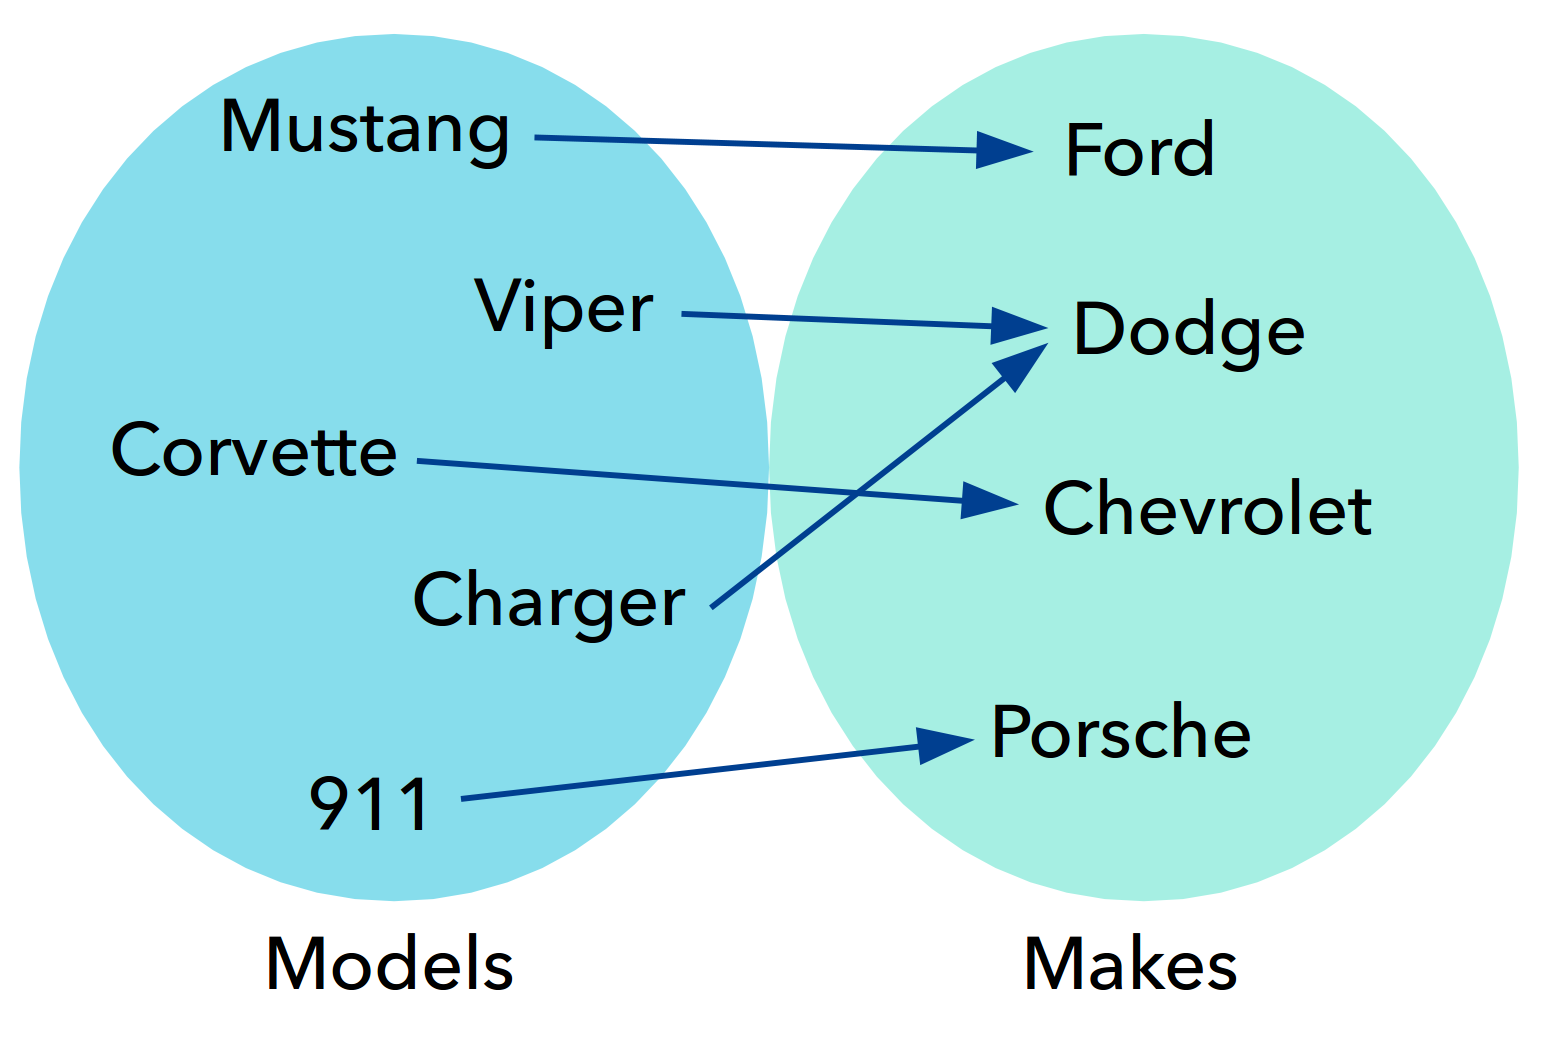
\includegraphics[0.8\textwidth]{./img/dict-01.png}
\end{frame}

%%%%%%%%%%%%%%%%%%%%%%%%%%%%%%%%%%%%%%%%%%%%%%%%%%%%%%%%%%%%%%%%%%%%%%%%%%%%%%%%
\begin{frame}[fragile]
  \frametitle{\texttt{dict} data type}
  \Enlarge

  \begin{itemize}
  \myitem  The \texttt{dict} indexes data by \emph{any} value (\emph{unordered}).
  \myitem  Easy to think of as dictionary, but can use lots besides strings.
  \myitem  This container maps \emph{keys} to \emph{values}.
  \end{itemize}
  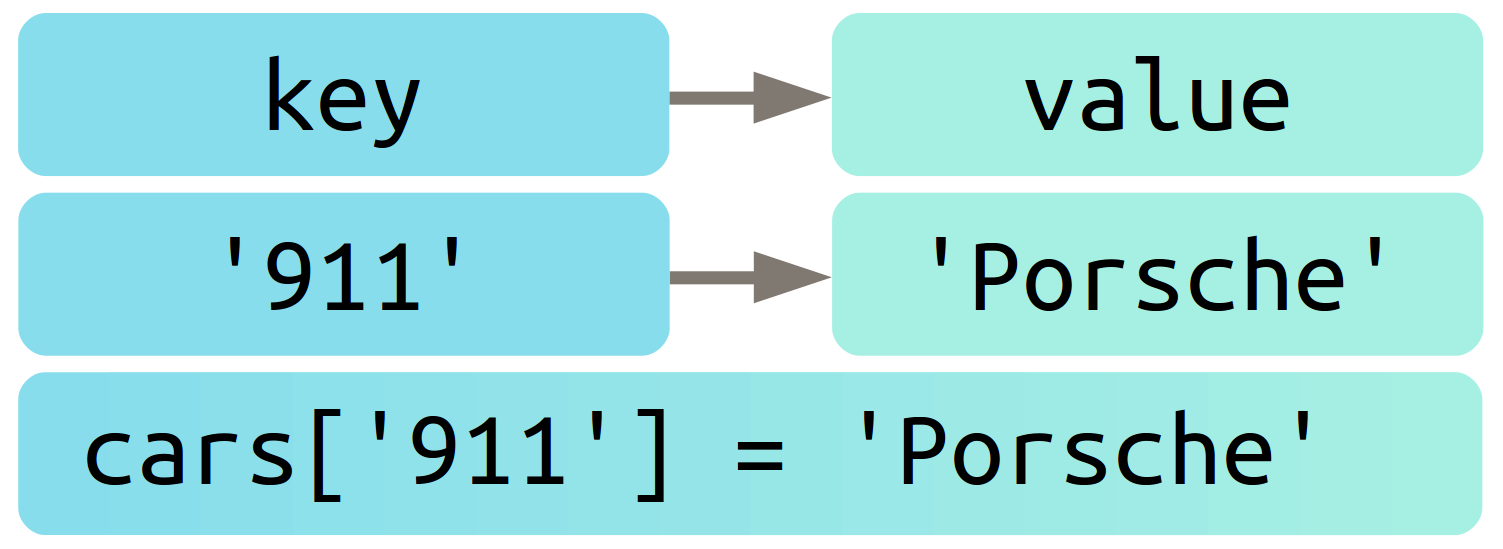
\includegraphics[0.8\textwidth]{./img/dict-02.png}
\end{frame}

%%%%%%%%%%%%%%%%%%%%%%%%%%%%%%%%%%%%%%%%%%%%%%%%%%%%%%%%%%%%%%%%%%%%%%%%%%%%%%%%
\begin{frame}[fragile]
  \frametitle{\texttt{dict} data type}
  \Enlarge

  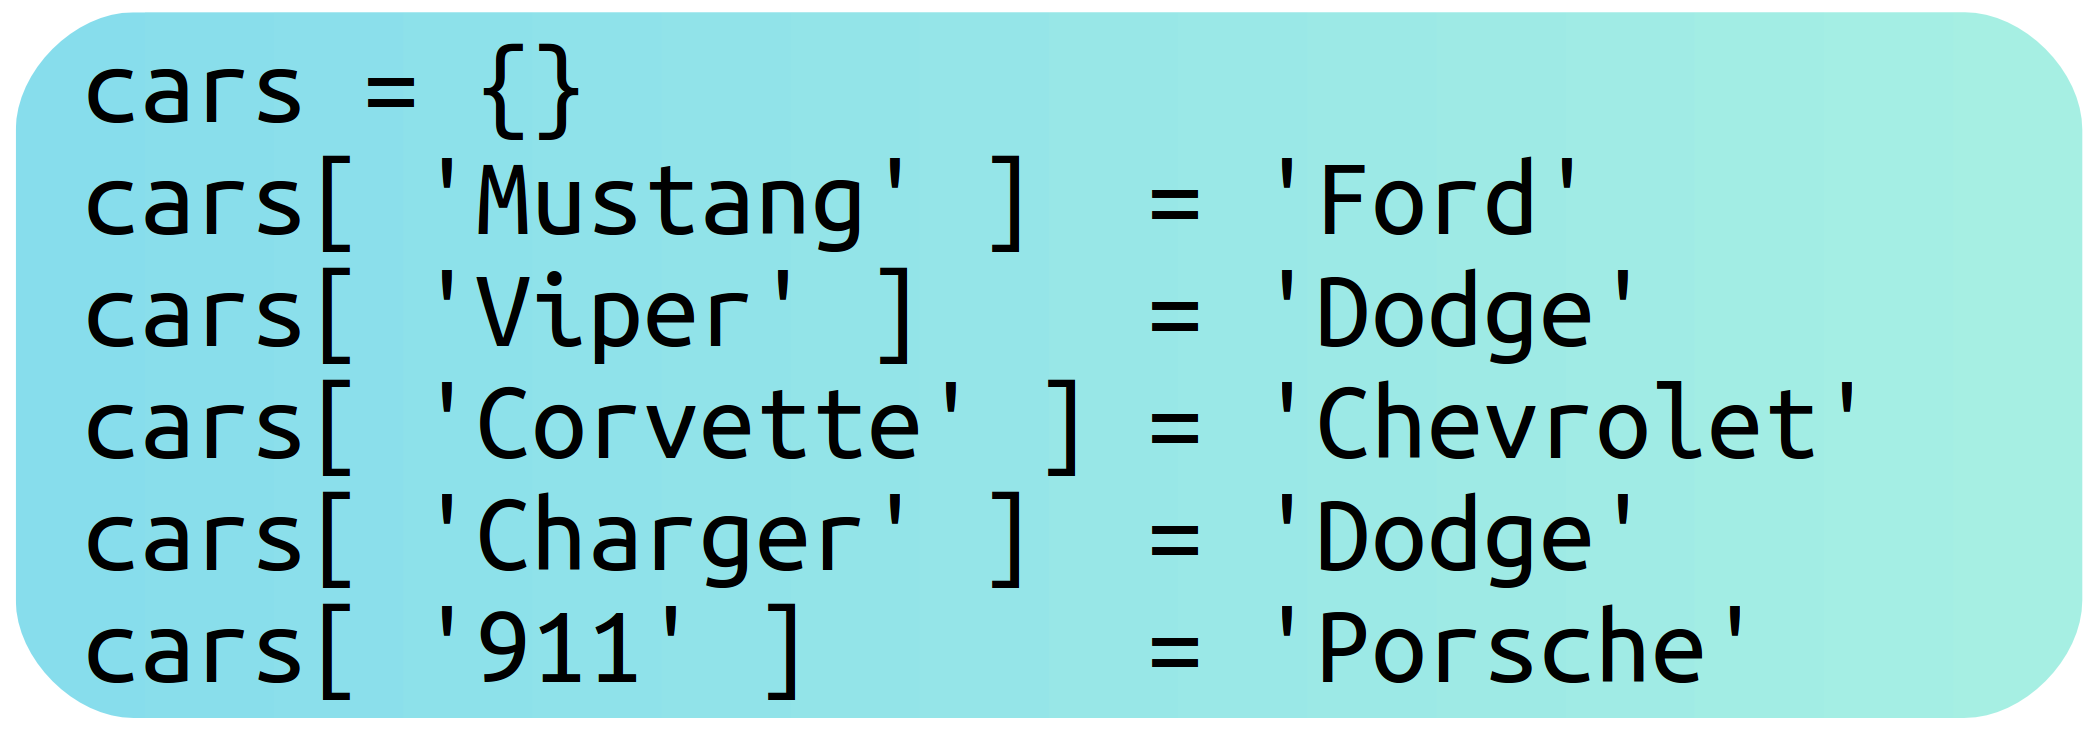
\includegraphics[0.8\textwidth]{./img/dict-03.png}
\end{frame}

%%%%%%%%%%%%%%%%%%%%%%%%%%%%%%%%%%%%%%%%%%%%%%%%%%%%%%%%%%%%%%%%%%%%%%%%%%%%%%%%
\begin{frame}[fragile]
  \frametitle{\texttt{dict} literals}
  \Enlarge

  \begin{itemize}
  \myitem  We create a \texttt{dict} as follows:
    \begin{itemize}
    \mysubitem  opening brace \texttt{\{}
    \mysubitem  \texttt{key : value} pairs, separated by commas
    \mysubitem  closing brace \texttt{\}}
    \end{itemize}
  \end{itemize}
  \begin{semiverbatim}
model = \{
  'Civic': 'Honda',
  'Mustang': 'Ford',
  'Model S': 'Tesla',
  'Model T': 'Ford'
\}
  \end{semiverbatim}
\end{frame}

%%%%%%%%%%%%%%%%%%%%%%%%%%%%%%%%%%%%%%%%%%%%%%%%%%%%%%%%%%%%%%%%%%%%%%%%%%%%%%%%
\begin{frame}[fragile]
  \frametitle{\texttt{dict} operations \& methods}
  \Enlarge

  \begin{semiverbatim}
d = \{ 'one':1, 'two':2, 'three':3 \}
print( d['one'] )
d[ 'four' ] = 4
del d[ 'four' ]
'five' in d
for key in d:  # no guarantee on order
    print( key, d[key] )
d.keys()
d.values()
  \end{semiverbatim}
\end{frame}

%%%%%%%%%%%%%%%%%%%%%%%%%%%%%%%%%%%%%%%%%%%%%%%%%%%%%%%%%%%%%%%%%%%%%%%%%%%%%%%%
\begin{frame}[fragile]
  \frametitle{Example}
  \Enlarge

  \begin{semiverbatim}
d = \{ 'a':2, 'c':3, 'b':1 \}
x = d[ 'a' ] + d[ 'c' ]
  \end{semiverbatim}
  What is the final value of \texttt{x}?
  \begin{enumerate}[label=\Alph*]
  \item  \texttt{4}
  \item  \texttt{'ac'}
  \item  \texttt{'5'}
  \item  \texttt{5}
  \end{enumerate}
\end{frame}

%%%%%%%%%%%%%%%%%%%%%%%%%%%%%%%%%%%%%%%%%%%%%%%%%%%%%%%%%%%%%%%%%%%%%%%%%%%%%%%%
\begin{frame}[fragile]
  \frametitle{Example}
  \Enlarge

  \begin{semiverbatim}
d = \{ \}
words = [ 'red', 'orange', 'yellow' ]
for word in words:
    d[ word ] = words.index( word )
  \end{semiverbatim}
  What is the final value of \texttt{d}?
  \begin{enumerate}[label=\Alph*]
  \item  \texttt{\{ 'red':3, 'orange':6, 'yellow':6 \}}
  \item  \texttt{\{ 'red':0, 'orange':2, 'yellow':2 \}}
  \item  \texttt{None}
  \item  \texttt{\{'orange': 1, 'red': 0, 'yellow': 2\}}
  \end{enumerate}
\end{frame}

%%%%%%%%%%%%%%%%%%%%%%%%%%%%%%%%%%%%%%%%%%%%%%%%%%%%%%%%%%%%%%%%%%%%%%%%%%%%%%%%
\begin{frame}[fragile]
  \frametitle{\texttt{dict} applications}
  \Enlarge

  \begin{itemize}
  \myitem  Dictionaries can encode/decode data, or translate from one representation to another.
  \end{itemize}
  \begin{semiverbatim}
x = 'ABCDEFGHIJKLMNOPQRSTUVWXYZ'
y = 'BCDEFGHIJKLMNOPQRSTUVWXYZA'
e = \{ \}
for i in range( len(x) ):
    e[ x[i] ] = y[i]
encoded = ''
for c in 'HELLO':
    encoded += e[c]
  \end{semiverbatim}
  \begin{itemize}
  \myitem  How would you reverse (decode) this?
  \end{itemize}
\end{frame}

%%%%%%%%%%%%%%%%%%%%%%%%%%%%%%%%%%%%%%%%%%%%%%%%%%%%%%%%%%%%%%%%%%%%%%%%%%%%%%%%
\begin{frame}[fragile]
  \frametitle{\texttt{dict} applications}
  \Enlarge

  \begin{semiverbatim}
x = 'ABCDEFGHIJKLMNOPQRSTUVWXYZ'
y = 'BCDEFGHIJKLMNOPQRSTUVWXYZA'
d = \{ \}
for i in range( len(x) ):
    d [y[i] ] = x[i]
decoded = ''
for c in encoded:
    decoded += d[c]
  \end{semiverbatim}
\end{frame}

%%%%%%%%%%%%%%%%%%%%%%%%%%%%%%%%%%%%%%%%%%%%%%%%%%%%%%%%%%%%%%%%%%%%%%%%%%%%%%%%
\begin{frame}[fragile]
  \frametitle{Exercise}
  \Enlarge

  \begin{itemize}
  \myitem  Encode all of the words in a file using a Caesar cipher.
  \myitem  Decode all of the words in the file.
  \end{itemize}
\end{frame}

%%%%%%%%%%%%%%%%%%%%%%%%%%%%%%%%%%%%%%%%%%%%%%%%%%%%%%%%%%%%%%%%%%%%%%%%%%%%%%%%
\begin{frame}[fragile]
  \frametitle{\texttt{dict} applications}
  \Enlarge

  \begin{itemize}
  \myitem  Dictionaries can also function as accumulators.
  \end{itemize}
  \begin{semiverbatim}
x = 'ABBACAB'
d = \{ \}
for c in x:
    if c not in d:
        d[c] = 0
        d[c] += 1
  \end{semiverbatim}
  \begin{itemize}
  \myitem  How would you reverse (decode) this?
  \end{itemize}
\end{frame}

%%%%%%%%%%%%%%%%%%%%%%%%%%%%%%%%%%%%%%%%%%%%%%%%%%%%%%%%%%%%%%%%%%%%%%%%%%%%%%%%
\begin{frame}[fragile]
  \frametitle{Exercise}
  \Enlarge

  \begin{itemize}
  \myitem  Count category frequencies in Jeopardy questions.
  \myitem  Count bigram frequencies in Jeopardy clues.
  \end{itemize}
\end{frame}

%%%%%%%%%%%%%%%%%%%%%%%%%%%%%%%%%%%%%%%%%%%%%%%%%%%%%%%%%%%%%%%%%%%%%%%%%%%%%%%%
\begin{frame}[fragile]
  \frametitle{\texttt{dict} applications}
  \Enlarge

  \begin{itemize}
  \myitem  We can link data based on a common field.
  \end{itemize}
  \begin{semiverbatim}
zipcode = \{ 'Bill': 60644,
            'Jill': 41073,
            'Tony': 63103 \}
city = \{ 60644: 'Chicago',
         41073: 'Cincinnati',
         63103: 'St. Louis' \}
for name in zipcode:
    print( name,city[zipcode[name]] )
  \end{semiverbatim}
\end{frame}

%%%%%%%%%%%%%%%%%%%%%%%%%%%%%%%%%%%%%%%%%%%%%%%%%%%%%%%%%%%%%%%%%%%%%%%%%%%%%%%%
\section{Mutable Arguments}

%%%%%%%%%%%%%%%%%%%%%%%%%%%%%%%%%%%%%%%%%%%%%%%%%%%%%%%%%%%%%%%%%%%%%%%%%%%%%%%%
\begin{frame}[fragile]
  \frametitle{Exercise:  mutability}
  \Enlarge

  \begin{semiverbatim}
x = [ 3,2,1 ]
y = x
y.sort()
x.append( 0 )
  \end{semiverbatim}
  What is the final value of \texttt{x}?
  \begin{enumerate}[label=\Alph*]
  \item  \texttt{[ 3,2,1 ]}
  \item  \texttt{[ 1,2,3 ]}
  \item  \texttt{[ 1,2,3,0 ]}
  \item  \texttt{[ 0,1,2,3 ]}
  \end{enumerate}
\end{frame}

%%%%%%%%%%%%%%%%%%%%%%%%%%%%%%%%%%%%%%%%%%%%%%%%%%%%%%%%%%%%%%%%%%%%%%%%%%%%%%%%
\begin{frame}[fragile]
  \frametitle{Mutable arguments}
  \Enlarge

  \begin{itemize}
  \myitem  Mutability causes \texttt{list}s to work differently in functions.
  \myitem  \texttt{list}s used as arguments \emph{can be changed} by the function.
  \myitem  This is very useful!
  \end{itemize}
  \begin{semiverbatim}
def fun(q):
    q.append(3)

a = [ ]
for i in range(3):
    fun(a)
print(a)
  \end{semiverbatim}
\end{frame}

%%%%%%%%%%%%%%%%%%%%%%%%%%%%%%%%%%%%%%%%%%%%%%%%%%%%%%%%%%%%%%%%%%%%%%%%%%%%%%%%
\begin{frame}[fragile]
  \frametitle{Mutable arguments}
  \Enlarge

  \begin{semiverbatim}
def readfile(fname,a):
    for line in open(fname):
        a.append(line)

all_lines = []
readfile( 'file1.txt', all_lines )
readfile( 'file2.txt', all_lines )
  \end{semiverbatim}
\end{frame}

%%%%%%%%%%%%%%%%%%%%%%%%%%%%%%%%%%%%%%%%%%%%%%%%%%%%%%%%%%%%%%%%%%%%%%%%%%%%%%%%
\begin{frame}[fragile]
  \frametitle{Mutable arguments}
  \Enlarge

  \begin{semiverbatim}
def readfile(fname,a):
    for line in open(fname):
        a.append(line)

all_lines = []
for f in open(“filenames.txt”):
    readfile(f,all_lines)
  \end{semiverbatim}
\end{frame}

%%%%%%%%%%%%%%%%%%%%%%%%%%%%%%%%%%%%%%%%%%%%%%%%%%%%%%%%%%%%%%%%%%%%%%%%%%%%%%%%
\begin{frame}[fragile]
  \frametitle{Copying mutable values}
  \Enlarge

  \begin{itemize}
  \myitem  What if we \emph{want} a copy of a \texttt{list} (not an alias)?
  \myitem  Slice!
  \end{itemize}
  \begin{semiverbatim}
x = [ 3,2,1 ]
y = x[ : ]
y.sort()
print( x )
  \end{semiverbatim}
\end{frame}

%%%%%%%%%%%%%%%%%%%%%%%%%%%%%%%%%%%%%%%%%%%%%%%%%%%%%%%%%%%%%%%%%%%%%%%%%%%%%%%%
\begin{frame}[fragile]
  \frametitle{Copying mutable values}
  \Enlarge

  \begin{semiverbatim}
x = [ 1,2,3 ]
y = x[ : ]
y.append( 4 )
print( x == y )
  \end{semiverbatim}
\end{frame}

%%%%%%%%%%%%%%%%%%%%%%%%%%%%%%%%%%%%%%%%%%%%%%%%%%%%%%%%%%%%%%%%%%%%%%%%%%%%%%%%
\section{String/List Methods}

%%%%%%%%%%%%%%%%%%%%%%%%%%%%%%%%%%%%%%%%%%%%%%%%%%%%%%%%%%%%%%%%%%%%%%%%%%%%%%%%
\begin{frame}[fragile]
  \frametitle{\texttt{string.split} method}
  \Enlarge

  \begin{itemize}
  \myitem  \texttt{split} returns a \texttt{list}.
  \myitem  Takes a single string argument, the \emph{delimiter}.
  \end{itemize}
  \begin{semiverbatim}
name = 'Oliver Wendell Holmes'
names = name.split(' ')
print(m[-1])
  \end{semiverbatim}
\end{frame}

%%%%%%%%%%%%%%%%%%%%%%%%%%%%%%%%%%%%%%%%%%%%%%%%%%%%%%%%%%%%%%%%%%%%%%%%%%%%%%%%
\begin{frame}[fragile]
  \frametitle{Example}
  \Enlarge

  \begin{semiverbatim}
x = 'A+B+C'
y = x.split('+')
  \end{semiverbatim}
  What is the final value of \texttt{y}?
  \begin{enumerate}[label=\Alph*]
  \item  \texttt{'ABC'}
  \item  \texttt{[ 'A','B','C' ]}
  \item  \texttt{'A','B','C'}
  \item  \texttt{None}
  \end{enumerate}
\end{frame}

%%%%%%%%%%%%%%%%%%%%%%%%%%%%%%%%%%%%%%%%%%%%%%%%%%%%%%%%%%%%%%%%%%%%%%%%%%%%%%%%
\begin{frame}[fragile]
  \frametitle{Example}
  \Enlarge

  \begin{semiverbatim}
x = 'A+B+C'
y = x.split('-')
  \end{semiverbatim}
  What is the final value of \texttt{y}?
  \begin{enumerate}[label=\Alph*]
  \item  \texttt{'A+B+C'}
  \item  \texttt{[ 'A+B+C' ]}
  \item  \texttt{( 'A+B+C' )}
  \item  \texttt{None}
  \end{enumerate}
\end{frame}

%%%%%%%%%%%%%%%%%%%%%%%%%%%%%%%%%%%%%%%%%%%%%%%%%%%%%%%%%%%%%%%%%%%%%%%%%%%%%%%%
\begin{frame}[fragile]
  \frametitle{\texttt{string.join} method}
  \Enlarge

  \begin{itemize}
  \myitem  \texttt{join} returns a \texttt{str}.
  \myitem  Takes a single \texttt{list} argument.
  \myitem  Returns the \texttt{list} elements joined as a string.
  \end{itemize}
  \begin{semiverbatim}
names = [ "Geoffrey", "Richard", "Aloysius", "Johnston", "Windsor", "Dean" ]
','.join(names)     # note the odd syntax!
  \end{semiverbatim}
\end{frame}

%%%%%%%%%%%%%%%%%%%%%%%%%%%%%%%%%%%%%%%%%%%%%%%%%%%%%%%%%%%%%%%%%%%%%%%%%%%%%%%%
\begin{frame}[fragile]
  \frametitle{Example}
  \Enlarge

  \begin{semiverbatim}
a = [ 'X', 'A', 'G' ]
b = a[:]
a.sort()
x = ','.join(b)
  \end{semiverbatim}
  What is the final value of \texttt{x}?
  \begin{enumerate}[label=\Alph*]
  \item  \texttt{'XAG'}
  \item  \texttt{[ 'X,A,G' ]}
  \item  \texttt{'A,G,X'}
  \item  \texttt{',A,G,X,'}
  \end{enumerate}
\end{frame}

%%%%%%%%%%%%%%%%%%%%%%%%%%%%%%%%%%%%%%%%%%%%%%%%%%%%%%%%%%%%%%%%%%%%%%%%%%%%%%%%
\section{Reminders}

%%%%%%%%%%%%%%%%%%%%%%%%%%%%%%%%%%%%%%%%%%%%%%%%%%%%%%%%%%%%%%%%%%%%%%%%%%%%%%%%
\begin{frame}
  \frametitle{Reminders}
  \Enlarge

  \begin{itemize}
  \myitem  Homework \#5 is due Friday Sep.\ 30.
  \myitem  Midterm \#1 will be Monday Oct.\ 3.  (7 p.m.) \\ \textcolor{CS101GradBot}{No class on Monday, \\ Labs WILL be held all week. \\ Contact \texttt{cs101admin@cs.illinois.edu} for conflict exam.}
  \end{itemize}
\end{frame}

\end{document}
